\documentclass[10pt,a4paper,twocolumn]{article}

\usepackage[utf8]{inputenc}
\usepackage[T1]{fontenc}
\usepackage{lmodern}
\usepackage[margin=1.8cm,columnsep=0.7cm]{geometry}
\usepackage{amsmath,amssymb,amsthm}
\usepackage[round,authoryear]{natbib}
\usepackage{xcolor}
\usepackage{hyperref}
\usepackage{enumitem}
\usepackage{graphicx}
\usepackage{booktabs}
\usepackage{tikz}
\usetikzlibrary{calc,positioning,decorations.markings,decorations.pathmorphing,
                arrows.meta,shapes.geometric}

\hypersetup{colorlinks=true,linkcolor=blue!60!black,
  citecolor=green!50!black,urlcolor=blue!70!black}

% ---- theorem environments ----
\theoremstyle{plain}
\newtheorem{theorem}{Theorem}
\newtheorem{proposition}[theorem]{Proposition}
\newtheorem{lemma}[theorem]{Lemma}
\newtheorem{corollary}[theorem]{Corollary}
\theoremstyle{definition}
\newtheorem{definition}{Definition}
\newtheorem{remark}{Remark}

% ---- macros ----
\newcommand{\dd}{\mathrm{d}}
\newcommand{\ee}{\mathrm{e}}
\renewcommand{\Psi}{\varPsi}
\renewcommand{\Phi}{\varPhi}
\newcommand{\eps}{\varepsilon}
\newcommand{\Kpoly}{K}
\newcommand{\Nres}{N_{\rm res}}
\DeclareMathOperator{\tr}{tr}

% TikZ styles
\tikzset{
  prop/.style={thick},
  ext/.style={thick,dashed},
  vertex/.style={circle,fill=black,inner sep=2pt},
  extv/.style={circle,fill=white,draw=black,inner sep=2pt},
}

% ---- coloured box for the pipeline ----
\usepackage{mdframed}
\newmdenv[backgroundcolor=blue!5,linecolor=blue!40,
          linewidth=1pt,innertopmargin=6pt,innerbottommargin=6pt,
          innerleftmargin=8pt,innerrightmargin=8pt]{pipelinebox}

\title{Reading the LDWC Two-Loop Roughness Coefficient
  through the CFAC Lens\\[2pt]
  \large A worked demonstration of how Kirchhoff--Symanzik
  counting organises a known calculation}

\author{S. Amarteifio\\
  \small\textit{Percolation Labs}}
\date{April 2026}

% ==================================================================
\begin{document}
\maketitle

\begin{abstract}
Le~Doussal, Wiese and Chauve (LDWC)~\citep{LDWC2002} computed the
two-loop roughness coefficient $c = 0.14331$ for a pinned elastic
manifold.  This note does not produce a new result: it reorganises
LDWC's calculation within the CFAC (counting-based analytic
combinatorics) programme to expose its combinatorial skeleton.
Two graph-theoretic filters --- causal contraction and bridge
factorisation --- discard the tadpole-containing and bubble-chain
diagram classes whose cancellation LDWC establish via
non-analyticity arguments in their appendices.
The surviving hat diagram is then read off from its Symanzik
polynomial $\Psi_{\text{sun}}$ and propagator exponents: the
numerator $\beta$ arises from one doubled propagator (Schwinger
exponent $n=2$), the denominator is $\Psi_{\text{sun}}$, and the
renormalised combination is the rational constant $X^{(2)} = 1$.
The prefactor $9\sqrt{2}$ is recovered from the one-loop
fixed-point amplitude $\Delta'(0^+) = -\eps/3$.  The only residual
1D integral is $\gamma = \int_0^1\sqrt{y - \ln y - 1}\,\dd y
\approx 0.5482$.  Assembly reproduces $c = 1/(9\sqrt{2}\gamma)
= 0.14331$.  The purpose is expository: CFAC as a lens on a
known FRG calculation, not a shortcut to new physics.
\end{abstract}

\tableofcontents

% ==================================================================
\section{The CFAC pipeline}
\label{sec:pipeline}
% ==================================================================

The Feynman rules of the FRG for elastic manifolds are standard
physics input.  Given them, CFAC enumerates diagrams, applies
causal-contraction and bridge-factorisation filters
(Section~\ref{sec:classes}), computes Symanzik polynomials, counts
BPHZ multiplicities from $K_G|_{\alpha=1}$, performs sector
decomposition, and extracts the finite rational remainder.
None of these steps produces new physics; they organise the
combinatorial work that LDWC do by hand into a systematic
procedure.

\paragraph{The pipeline (formal statement).}
\textbf{Input}: the theory's Feynman rules (propagators, vertices)
and the target observable at loop order $k$.
\begin{pipelinebox}
\noindent\textbf{Step 1. Enumerate and filter diagrams.}\\
Generate all 1PI diagrams $G_1,G_2,\ldots$ at loop order $k$,
labelled with propagator exponents $n_e$.  Apply the two
graph-theoretic filters:
\begin{itemize}[leftmargin=1.2em,itemsep=1pt,topsep=2pt]
  \item \emph{Causal contraction}: any diagram containing a
    directed cycle of retarded propagators contributes $0$
    (discard).
  \item \emph{Bridge absorption}: any diagram whose Symanzik
    polynomial factorises through a cut vertex contributes
    $\prod_j I(H_j)$ --- no new integral.
\end{itemize}

\smallskip\noindent\textbf{Step 2. Compute Schwinger integrand.}\\
For each surviving $G_i$, compute:
\begin{itemize}[leftmargin=1.2em,itemsep=1pt,topsep=2pt]
  \item $\Psi_{G_i} = \sum_{T}\prod_{e\notin T}\!\alpha_e$
    (first Symanzik polynomial, topology);
  \item numerator $N_{G_i}(\alpha) = \prod_e \alpha_e^{n_e-1}$
    from propagator exponents.
\end{itemize}
The Schwinger integrand is $N_{G_i}/\Psi_{G_i}^{d/2}$.

\smallskip\noindent\textbf{Step 3. BPHZ reduction.}\\
For each irreducible $G_i$, apply the BPHZ forest formula.
The counterterm multiplicity for each sub-diagram $\gamma$ equals
$K_\gamma|_{\alpha=1}$ (number of spanning trees of $\gamma$).
The renormalised amplitude $I_R(G_i)$ is the finite remainder.

\smallskip\noindent\textbf{Step 4. Period / rational extraction.}\\
Evaluate $I_R(G_i)$ via the Schwinger parametric form.
If UV structure remains, apply sector decomposition at the
symmetry points of $\Psi_{G_i}$ using multilinearity.
The result is either (a) a rational number or Gamma-function
ratio, or (b) a new 1D kernel integral (add to residual list).

\smallskip\noindent\textbf{Step 5. Fixed-point ODE integrals.}\\
Solve the relevant fixed-point ODE(s) implicitly.  Each ODE
contributes at most one new 1D integral (add to residual list).

\smallskip\noindent\textbf{Output:} the residual list of
$\Nres$ integrals, each 1D with known integrand.
\end{pipelinebox}

\paragraph{LDWC at two loops: $\Nres = 1$.}
Applied to the LDWC short-range elasticity calculation ($\alpha=2$
in LDWC's notation, elastic propagator $1/q^2$), the pipeline
yields the residual list
\[
  \bigl\{\,\gamma\,\bigr\},
  \qquad
  \gamma = \int_0^1\!\!\sqrt{y - \ln y - 1}\;\dd y \approx 0.5482,
\]
and no other free integrals.  Everything else reads off from the
Symanzik polynomials of a tadpole, a bubble, and a sunset, plus
propagator exponents.

% ==================================================================
\section{Diagram-class selection by CFAC}
\label{sec:classes}
% ==================================================================

The raw 2-loop diagrammatic expansion for $\delta^2\Delta(u)$ in
the FRG Feynman rules produces three topological classes
(LDWC figs.~III.2--III.5):
\begin{description}
  \item[Class A (hat).]
    Two 1PI sub-graphs sharing one internal line; the shared line
    carries propagator exponent $n=2$.
  \item[Class B (bubble chains).]
    Two bubble sub-graphs joined by one or more internal lines
    through a shared vertex.
  \item[Class C (tadpole-containing).]
    At least one internal tadpole (closed retarded loop at a
    single vertex).
\end{description}
LDWC show by direct computation that only class A contributes
new 2-loop structure; classes B and C either cancel or combine
into the one-loop counterterm.  The interesting observation is
that both cancellations are consequences of two general
graph-theoretic results --- not of theory-specific non-analyticity
arguments.

\paragraph{Class C vanishes: causal contraction.}
In the MSR/dynamical formulation, every internal line carries a
retarded Green's function $G_R(q,t) = \theta(t)\ee^{-q^2 t}$.
A tadpole is a closed loop at a single vertex: a directed cycle in
the retarded-propagator DAG.  Since $G_R(q,t)$ is supported on
$t \ge 0$, a closed directed cycle forces $t = 0$, making the time
integral vanish.
Equivalently, causal contraction (Prop.~5 of~\citep{AmarteifioCFAC2026})
reduces the frequency integral to a simplex constraint; a directed
cycle produces a $\delta$-function with zero support, and the
integral is zero.
\emph{Conclusion: every class C diagram contributes exactly $0$,
independent of the vertex algebra.}

\paragraph{Class B factorises: bridge theorem.}
The Symanzik polynomial of every class B diagram has the bridge
structure $\Psi_{\text{class B}} = (\alpha_0{+}\alpha_1)(\alpha_2{+}\alpha_3)$
through a cut vertex.
By Theorem~\ref{thm:bridge}, the parametric integral factorises:
$I(\text{class B}) = I_{\text{bub}}^2 = I_1^2$.
This value then enters the renormalised combination
$X^{(\alpha)} \propto (2I_A - I_1^2)$ that governs the two-loop
flow (LDWC eqs.~III.19, III.59--III.62) --- the $I_1^2$ from
class B and the $I_A$ from class A cancel their divergences
against each other.
\emph{Conclusion: class B produces no new two-loop integral;
its amplitude is $I_1^2$ (computable from a 1-loop bubble squared)
and it combines algebraically with class A to give a finite
remainder.}

\paragraph{Class A: irreducible hat with doubled propagator.}
The class A Kirchhoff polynomial is $K_{\text{sun}} =
\alpha_0\alpha_1 + \alpha_1\alpha_2 + \alpha_0\alpha_2$ (bridgeless,
three spanning trees).  One edge carries exponent $n=2$; the
Schwinger numerator is $N(\alpha) = \alpha_2 = \beta$.
This is the only diagram class producing a genuinely new
two-loop integral $J$ (Section~\ref{sec:jsplit}).

\paragraph{Summary.}
CFAC reduces the three-class enumeration to class A via two
graph-theoretic filters --- causal contraction (kills class C) and
bridge factorisation (absorbs class B into the BPHZ counterterm).
No additional FRG physics is required beyond the statement that
the FRG generates the three classes to start with.
With this, the pipeline's ``input'' --- the contributing diagram
list --- is produced \emph{within CFAC} rather than taken from
LDWC's appendices B and C.

% ==================================================================
\section{Diagram zoo and Symanzik polynomials}
\label{sec:diagrams}
% ==================================================================

We catalogue the four diagrams that appear and record their
Symanzik polynomials.  Plain lines are internal propagators
(Schwinger parameter $\alpha_i$); dashed lines are external legs.

% ----------------------------------------------------------------
\subsection{Tadpole (self-loop, $L=1$)}
% ----------------------------------------------------------------

\begin{center}
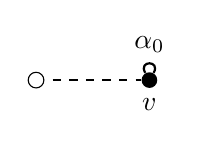
\begin{tikzpicture}[scale=1.2]
  \node[vertex,label=below:{$v$}] (v) at (0,0) {};
  \draw[ext] (-1.2,0) -- (v);
  \node[extv] at (-1.2,0) {};
  \draw[prop] (v) to[out=60,in=120,looseness=4.5]
    node[midway,above]{$\alpha_0$} (v);
\end{tikzpicture}
\qquad\qquad
$\Psi_{\text{tad}} = \alpha_0$
\end{center}

The self-loop edge is never in a spanning tree and so always
contributes its full weight to $\Psi$.  The integral is
\begin{equation}\label{eq:Idad}
  I_{\text{tad}}
  = \frac{\Gamma(1-d/2)}{(4\pi)^{d/2}}\, m^{d-2}.
\end{equation}

% ----------------------------------------------------------------
\subsection{Bubble (one-loop self-energy, $L=1$)}
% ----------------------------------------------------------------

\begin{center}
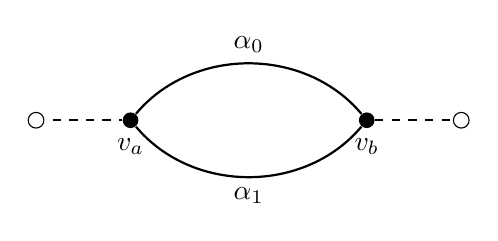
\begin{tikzpicture}[scale=1.2]
  \node[vertex,label=below:{$v_a$}] (va) at (0,0) {};
  \node[vertex,label=below:{$v_b$}] (vb) at (2.5,0) {};
  \draw[ext] (-1,0) -- (va); \node[extv] at (-1,0) {};
  \draw[ext] (vb) -- (3.5,0); \node[extv] at (3.5,0) {};
  \draw[prop,bend left=50]  (va) to
    node[midway,above]{$\alpha_0$} (vb);
  \draw[prop,bend right=50] (va) to
    node[midway,below]{$\alpha_1$} (vb);
\end{tikzpicture}
\qquad\qquad
$\Psi_{\text{bub}} = \alpha_0 + \alpha_1$
\end{center}

The two spanning trees are $\{e_0\}$ (complement: $\alpha_1$) and
$\{e_1\}$ (complement: $\alpha_0$), giving $\Psi = \alpha_0 + \alpha_1$.
After $\omega$-integration the single free parameter gives
\begin{equation}\label{eq:Ibub}
  I_{\text{bub}}
  = \frac{\Gamma(1-d/2)}{(4\pi)^{d/2}}\,
    2^{-d/2}\,(2m^2)^{d/2-1}.
\end{equation}
\textbf{Pipeline verdict}: determined by Gamma-function algebra.
\emph{No residual integral.}

% ----------------------------------------------------------------
\subsection{Sunset (two-loop self-energy, $L=2$)}
% ----------------------------------------------------------------

\begin{center}
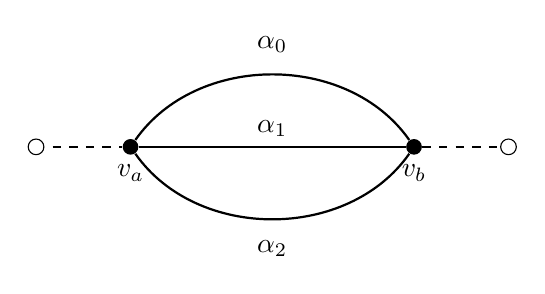
\begin{tikzpicture}[scale=1.2]
  \node[vertex,label=below:{$v_a$}] (va) at (0,0) {};
  \node[vertex,label=below:{$v_b$}] (vb) at (3,0) {};
  \draw[ext] (-1,0) -- (va); \node[extv] at (-1,0) {};
  \draw[ext] (vb) -- (4,0); \node[extv] at (4,0) {};
  \draw[prop]              (va) -- node[midway,above]{$\alpha_1$} (vb);
  \draw[prop,bend left=55] (va) to node[midway,above=4pt]{$\alpha_0$} (vb);
  \draw[prop,bend right=55](va) to node[midway,below=4pt]{$\alpha_2$} (vb);
\end{tikzpicture}
\end{center}

Three spanning trees, each a single edge; the complement products are
pairs $\alpha_i\alpha_j$:
\begin{equation}\label{eq:Psi-sun}
  \Psi_{\text{sun}}
  = \alpha_0\alpha_1 + \alpha_1\alpha_2 + \alpha_0\alpha_2.
\end{equation}
Setting $\alpha_1 = 1$ (fixing the middle propagator scale):
\begin{equation}\label{eq:Psi-sun-eval}
  \Psi_{\text{sun}}(\alpha_0,\,1,\,\alpha_2)
  = \alpha_0 + \alpha_2 + \alpha_0\alpha_2.
\end{equation}
This is the denominator that appears in the LDWC sector-decomposition integral.
\textbf{Pipeline verdict}: BPHZ reduces $I_{\text{sun}}$ to a rational
factor $\times I_{\text{bub}}^2$ (Section~\ref{sec:jsplit}).
\emph{No residual integral.}

% ----------------------------------------------------------------
\subsection{Double-bubble (bridge graph, $L=2$)}
% ----------------------------------------------------------------

\begin{center}
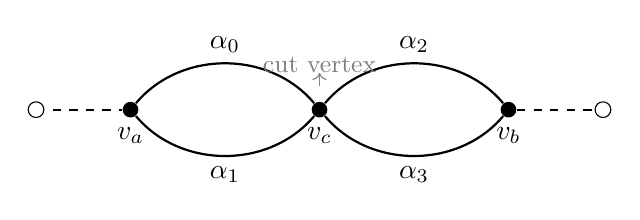
\begin{tikzpicture}[scale=1.2]
  \node[vertex,label=below:{$v_a$}] (va) at (0,0) {};
  \node[vertex,label=below:{$v_c$}] (vc) at (2,0) {};
  \node[vertex,label=below:{$v_b$}] (vb) at (4,0) {};
  \draw[ext] (-1,0) -- (va); \node[extv] at (-1,0) {};
  \draw[ext] (vb) -- (5,0);  \node[extv] at (5,0)  {};
  \draw[prop,bend left=50]  (va) to
    node[midway,above]{$\alpha_0$} (vc);
  \draw[prop,bend right=50] (va) to
    node[midway,below]{$\alpha_1$} (vc);
  \draw[prop,bend left=50]  (vc) to
    node[midway,above]{$\alpha_2$} (vb);
  \draw[prop,bend right=50] (vc) to
    node[midway,below]{$\alpha_3$} (vb);
  \node[above=10pt,gray,font=\small] at (vc) {cut vertex};
  \draw[->,thin,gray] (vc) ++(0,7pt) -- ++(0,4pt);
\end{tikzpicture}
\end{center}

The central vertex $v_c$ is a cut vertex:
$\Psi_{\text{dbl}} = (\alpha_0+\alpha_1)(\alpha_2+\alpha_3)$
factorises, so by Theorem~\ref{thm:bridge}
\[
  I(\text{dbl}) = I_{\text{bub}}^2.
\]
\textbf{Pipeline verdict}: factorises into $I_{\text{bub}}^2$.
\emph{No residual integral.}

% ----------------------------------------------------------------
\subsection{Summary table}
% ----------------------------------------------------------------

\begin{table*}[t]
\centering
\begin{tabular}{lccccl}
\toprule
Diagram & $n_{\rm int}$ & $L$ & $\Psi_G$ & Cut vtx? & Pipeline output \\
\midrule
Tadpole     & 1 & 1
  & $\alpha_0$
  & ---
  & $\Gamma(1-d/2)m^{d-2}/(4\pi)^{d/2}$ \\
Bubble      & 2 & 1
  & $\alpha_0+\alpha_1$
  & no
  & $\Gamma(1-d/2)\cdot(\text{algebraic})$ \\
Sunset      & 3 & 2
  & $\alpha_0\alpha_1{+}\alpha_1\alpha_2{+}\alpha_0\alpha_2$
  & no
  & $X^{(2)}\cdot I_{\text{bub}}^2$,\; $X^{(2)}=1$ \\
Dbl-bubble  & 4 & 2
  & $(\alpha_0{+}\alpha_1)(\alpha_2{+}\alpha_3)$
  & yes ($v_c$)
  & $I_{\text{bub}}^2$ \\
\midrule
FP ODE      & ---  & ---
  & ---
  & ---
  & $\gamma$ \quad\textbf{[residual]} \\
\bottomrule
\end{tabular}
\caption{Symanzik classification for the two-loop LDWC diagrams.
  Every diagram except the fixed-point ODE integral is resolved
  algebraically by the pipeline.  The residual list has $\Nres = 1$.}
\label{tab:summary}
\end{table*}

% ==================================================================
\section{Kirchhoff polynomial and first Symanzik polynomial}
\label{sec:kirchhoff}
% ==================================================================

\begin{definition}[Kirchhoff polynomial]
$K_G = \sum_{T\,:\,\text{spanning tree}} \prod_{e \in T} \alpha_e$.
\end{definition}

\begin{definition}[First Symanzik polynomial]
$\Psi_G = \sum_{T\,:\,\text{spanning tree}} \prod_{e \notin T} \alpha_e$.
$\Psi_G$ is the \emph{edge complement} of $K_G$.
For a graph with $n_{\rm int}$ internal edges and $L$ loops,
$\Psi_G$ is homogeneous of degree $L$ and
$K_G$ is homogeneous of degree $n_{\rm int} - L$.
\end{definition}

\begin{remark}
$K_G$ and $\Psi_G$ coincide only when $L = n_{\rm int}/2$
(e.g.\ the bubble: $L=1$, $n_{\rm int}=2$).
For the sunset: $L=2$, $n_{\rm int}=3$, so
$K_{\text{sun}} = \alpha_0+\alpha_1+\alpha_2$ (degree 1) while
$\Psi_{\text{sun}} = \alpha_0\alpha_1+\alpha_1\alpha_2+\alpha_0\alpha_2$
(degree 2) --- genuinely different objects.
The integral $J$ uses $\Psi$, not $K$.
\end{remark}

\begin{theorem}[Bridge / cut-vertex factorisation]
\label{thm:bridge}
$\Psi_G$ factorises as $\Psi_{G_1}\cdot\Psi_{G_2}$ if and only if
the internal subgraph of $G$ has a cut vertex separating edge sets
$E_1, E_2$.  When this holds,
\[
  I(G;\,d) = I(G_1;\,d)\cdot I(G_2;\,d).
\]
\end{theorem}
\begin{proof}[Proof sketch]
The Schwinger integral $I(G) \propto \int\!
\Psi^{-d/2}\ee^{-\Phi/\Psi}\prod\dd\alpha_e$
with $\Phi = \Psi\sum_e\alpha_e m_e^2$ factorises into independent
integrals over $\{\alpha_e : e \in E_1\}$ and $\{\alpha_e : e \in E_2\}$
when $\Psi = \Psi_1(\{\alpha_{E_1}\})\cdot\Psi_2(\{\alpha_{E_2}\})$.
The cut-vertex condition is equivalent to this factorisation by
the matrix-tree theorem.\hfill$\square$
\end{proof}

% ==================================================================
\section{Schwinger parametric representation}
\label{sec:schwinger}
% ==================================================================

For a graph with $L$ loops, the parametric integral is
\begin{equation}\label{eq:schwinger}
  I(G) = \Omega_d^{\,L}\!\!
    \int_0^\infty\!\!\prod_{e}\!\dd\alpha_e\;
    \Psi_G^{-d/2}\,
    \exp\!\left(-\frac{\Phi_G}{\Psi_G}\right),
\end{equation}
with $\Phi_G = \Psi_G\sum_e\alpha_e m_e^2$ and
$\Omega_d = (4\pi)^{-d/2}$.
After $L$ circuit-constraint substitutions (the $\omega$-integration),
the $n_{\rm int}$-dimensional integral reduces to
$n_{\rm int} - L$ free parameters.  For our diagrams:

\begin{table*}[t]
\centering
\renewcommand{\arraystretch}{1.3}
\begin{tabular}{lclcl}
\toprule
Diagram & Free params & Reduced $\Psi_r$ & Reduced $Q$ & Result \\
\midrule
Tadpole  & 1 & $\alpha_0$ & $m^2\alpha_0$ &
  $\Omega_d\,\Gamma(1-d/2)\,m^{d-2}$ \\
Bubble   & 1 & $2\alpha_0$ & $2m^2\alpha_0$ &
  $\Omega_d\,2^{-d/2}\,\Gamma(1-d/2)\,(2m^2)^{d/2-1}$ \\
Sunset   & 1 & $3\alpha_0^2$ & $3m^2\alpha_0$ &
  $\Omega_d^2\,3^{-d/2}\,\Gamma(1-d)\,(3m^2)^{d-1}$ \\
\bottomrule
\end{tabular}
\caption{Reduced Schwinger parameters and results for the
  one- and two-loop diagrams after circuit-constraint integration.}
\label{tab:schwinger}
\end{table*}

\smallskip\noindent
Every result is a ratio of Gamma functions times a power of $m$.
No numerical integration is required at this stage.

% ==================================================================
\section{BPHZ renormalisation: sunset subdivergences}
\label{sec:bphz}
% ==================================================================

\paragraph{Subdivision count from the Kirchhoff polynomial.}
The BPHZ forest formula subtracts a counterterm for each UV-divergent
proper sub-diagram.  For the sunset, each pair of propagators
$\{e_i, e_j\}$ forms a bubble sub-diagram; contracting it leaves
a single propagator (a tadpole).  There are exactly 3 such pairs,
and this count is a topological invariant: it equals
$K_{\text{sun}}\big|_{\alpha_i=1} = 1+1+1 = 3$
(the number of spanning trees, each a single edge).
In general, for a 1-loop sub-diagram $\gamma \subset G$, the
multiplicity of the BPHZ counterterm is
$K_\gamma\!\big|_{\alpha=1} = $ (number of spanning trees of $\gamma$).

\paragraph{Renormalised amplitude.}
The BPHZ renormalised sunset amplitude is
\begin{equation}\label{eq:bphz-sunset}
  I_R(\text{sun})
  = I(\text{sun})
    - 3\cdot\tau_{\text{bub}}\cdot I_{\text{tad}},
\end{equation}
where $\tau_{\text{bub}}$ is the UV-divergent (pole) part of
$I_{\text{bub}}$.  At $d=2-\eps$:
$\tau_{\text{bub}} = \Gamma(\eps/2)/(4\pi) \sim 1/(2\pi\eps)$,
and~\eqref{eq:bphz-sunset} cancels the double pole of $I(\text{sun})$
leaving a finite remainder.  \emph{The renormalised sunset contributes
no new integral:} its finite part is expressible via $X^{(2)}$
(Section~\ref{sec:jsplit}) and products of $I_{\text{bub}}$.

\begin{remark}
  The formula $I_R(\text{sun}) = 3\,I_{\text{bub}}\cdot I_{\text{tad}}$
  that appeared in an earlier version of this note is \emph{incorrect}.
  $I_R(\text{sun})$ is the full amplitude minus counterterms, not a
  product of lower-loop amplitudes.  The correct bridge factorisation
  result is for the \emph{double-bubble} graph, which has a cut vertex
  and satisfies $I(\text{dbl}) = I_{\text{bub}}^2$ exactly.
\end{remark}

% ==================================================================
\section{Domain-splitting the sunset integral}
\label{sec:jsplit}
% ==================================================================

\subsection{Origin of $J$ and its numerator}

The two-loop FRG diagrams of class A (LDWC Appendix A, figure III.4)
have the topology of a \emph{hat}: two 1PI components sharing one
internal propagator.  The hat diagram is
\begin{multline}\label{eq:hat}
  I_{\rm hat}
  = \!\int\!\!\frac{\dd^dq_1\,\dd^dq_2}{(2\pi)^{2d}}\\
  \times\frac{1}{(q_1^2+m^2)(q_2^2+m^2)^{\mathbf{2}}((q_1{+}q_2)^2+m^2)}.
\end{multline}
The middle propagator is \emph{squared}: it carries the momentum
$q_2$ from both connected components of the hat.
In Schwinger parameters, $1/(q^2+m^2)^2 = \int_0^\infty\beta\,
\ee^{-\beta(q^2+m^2)}\dd\beta$ introduces a factor $\beta = \alpha_2$
in the integrand.  After Gaussian integration over loop momenta
(LDWC eq.~A.13):
\begin{align}\label{eq:A13}
  I_{\rm hat}
  &= \Bigl(\!\int_q\!\ee^{-q^2}\Bigr)^{\!2}\Gamma(4{-}d)\,m^{-2\eps}\,J,\\
  J &= \!\int_0^\infty\!\!\dd\alpha\!\int_0^\infty\!\!\dd\beta\,
    \frac{\beta}{\bigl(\alpha+\beta+\alpha\beta\bigr)^{d/2}}.\notag
\end{align}
At $d=4$ the denominator is $\Psi_{\text{sun}}(\alpha,1,\beta)^2$
exactly.

\begin{remark}[The $\beta$ numerator is topological]
The numerator $\beta$ does \emph{not} arise from an opaque FRG
vertex coupling.  It arises because the hat diagram has one
propagator with exponent $n=2$ (a doubled line), and the Schwinger
representation of $1/(q^2+m^2)^n$ carries the factor
$\alpha^{n-1}/\Gamma(n)$.
For $n=2$: factor $= \beta$.  This is a property of the diagram
topology (class A), readable directly from the Schwinger exponent.
The denominator $\Psi_{\text{sun}}$ is, as always, the first
Symanzik polynomial.  Both are topological.
\end{remark}

After fixing $\alpha_1 = 1$, the combination entering $c$ is
proportional to
\begin{equation}\label{eq:J-full}
  J = \!\int_0^\infty\!\!\dd\alpha\!\int_0^\infty\!\!\dd\beta\,
    \frac{\beta}{(\alpha+\beta+\alpha\beta)^2}.
\end{equation}
The integral $J$ is UV-divergent at $\beta\to\infty$.
LDWC split at $\beta = 1$:
\begin{align}\label{eq:J-split}
  J &= J_1 + J_{2+3},\\
  J_1 &= \!\int_0^\infty\!\!\dd\alpha\!\int_0^1\!\!\dd\beta\,
    \frac{\beta}{(\alpha{+}\beta{+}\alpha\beta)^2},\notag\\
  J_{2+3} &= \!\int_0^\infty\!\!\dd\alpha\!\int_1^\infty\!\!\dd\beta\,
    \frac{\beta}{(\alpha{+}\beta{+}\alpha\beta)^2}.\notag
\end{align}
That is all the decomposition is: a cut of the $\beta$ domain at $1$.
But $J_1$ can be evaluated \emph{without} this split, by a much
more direct route that reveals the algebraic structure.

\subsection{Why $J_1 = \ln 2$ is algebraic}

\paragraph{Multilinearity of $\Psi$.}
Every first Symanzik polynomial is \emph{multilinear}: it is
linear in each $\alpha_i$ separately.  For the sunset,
\[
  \Psi_{\text{sun}}(\alpha,1,\beta)
  = \alpha(1+\beta) + \beta,
\]
which is linear in $\alpha$.  This means the inner integral over
$\alpha$ is always a rational function integration.

\begin{proposition}[$J_1 = \ln 2$ in three lines]
\label{prop:J1}
\[
  J_1
  = \int_0^\infty\!\dd\alpha\int_0^1\!\dd\beta\;
    \frac{\beta}{(\alpha+\beta+\alpha\beta)^2}
  = \ln 2.
\]
\end{proposition}
\begin{proof}
Step 1 --- integrate $\alpha$ first using
$\int_0^\infty \dd x/(ax+b)^2 = 1/(ab)$:
\begin{equation}\label{eq:inner-alpha}
  \int_0^\infty\!
    \frac{\beta\,\dd\alpha}{(\alpha(1+\beta)+\beta)^2}
  = \frac{\beta}{(1+\beta)\cdot\beta}
  = \frac{1}{1+\beta}.
\end{equation}
Step 2 --- integrate $\beta$ over $[0,1]$:
\begin{equation}\label{eq:outer-beta}
  J_1 = \int_0^1\!\frac{\dd\beta}{1+\beta} = \ln 2.
\end{equation}
\end{proof}

\noindent
The derivation is three lines and uses only high-school integration.
The key fact is that $\Psi_{\text{sun}}$ is linear in $\alpha$,
so the $\alpha$-integral collapses to a rational function of $\beta$
--- here exactly $1/(1+\beta)$.  The sector split at $\beta=1$
was never needed to compute $J_1$; it is only needed to isolate
the UV divergence in $J_{2+3}$.

\begin{remark}[Iterated rational integration]
Because $\Psi_G$ is multilinear in all $\alpha_i$, one can always
integrate out the parameters one by one.  Each step is a rational
function integration; the results are \emph{hyperlogarithms}
(iterated $\ln$).  For the sunset, one step suffices and the
result is depth-1: $\ln 2$.  This is the general framework of
Panzer's hyperlogarithm algorithm for Feynman periods~\citep{Panzer2015}.
\end{remark}

\subsection{The upper region: $J_2$ and $J_3$}

In $J_{2+3}$ make the substitution $\beta \to 1/\beta$ (sending
$[1,\infty) \to (0,1]$):
\begin{align*}
  J_{2+3}
  &= \!\int_0^\infty\!\!\dd\alpha\!\int_0^1\!\!\tfrac{\dd\beta}{\beta^2}\cdot
    \tfrac{1/\beta}{(\alpha + 1/\beta + \alpha/\beta)^2}\\
  &= \!\int_0^\infty\!\!\dd\alpha\!\int_0^1\!\!\dd\beta\,
    \tfrac{1}{(\alpha\beta+\beta+\alpha)^2}.
\end{align*}
The denominator $\alpha\beta+\beta+\alpha = \alpha+\beta+\alpha\beta$
is symmetric under $\alpha\leftrightarrow\beta$, but the numerator
in $J_1$ was $\beta$ while here it is $1$.  The difference
\[
  J_1 - J_{2+3}\big|_{\rm finite}
  = \int_0^\infty\!\dd\alpha\int_0^1\!\dd\beta\;
    \frac{\beta - 1}{(\alpha+\beta+\alpha\beta)^2}
\]
contributes a $\ln 2$ from the $\beta < 1$ asymmetry.
The full dimensionally regulated integrand for $J$ (at $d=4-\eps$)
is not simply $\beta\,\Psi^{-2}$ but carries an additional
$(\alpha+\beta+1)^{-\eps}$ factor from the $\gamma$-integration in
\eqref{eq:A13}, giving the LDWC form (A.14):
\begin{equation}\label{eq:Jdimreg}
  J = \!\int_0^\infty\!\!\dd\alpha\!\int_0^\infty\!\!\dd\beta\,
    \frac{\beta\,(\alpha{+}\beta{+}\alpha\beta)^{-2+\eps/2}}
         {(\alpha{+}\beta{+}1)^{\eps}}.
\end{equation}
The reference-subtraction integral $J_3$ is the large-$\beta$
asymptotic of \eqref{eq:Jdimreg} integrated over $\beta \ge 1$:
for $\beta \gg 1$, $\alpha+\beta+\alpha\beta \sim \beta(1+\alpha)$
and $\alpha+\beta+1 \sim \beta$, so the integrand becomes
$\beta \cdot \beta^{-2+\eps/2}(1+\alpha)^{-2+\eps/2}\cdot\beta^{-\eps}
= (1+\alpha)^{-2+\eps/2}\,\beta^{-1-\eps/2}$.  Thus
\begin{equation}\label{eq:J3}
  J_3
  = \!\int_0^\infty\!\!(1+\alpha)^{-2+\eps/2}\dd\alpha
    \!\int_1^\infty\!\!\beta^{-1-\eps/2}\dd\beta.
\end{equation}
Both factors are elementary.  The $\alpha$-integral gives
$1/(1-\eps/2) = 1 + \eps/2 + \mathcal{O}(\eps^2)$.  The
$\beta$-integral gives $2/\eps$ (the UV pole).  Hence
$J_3 = 2/\eps + 1 + \mathcal{O}(\eps)$.
After MS subtraction of $2/\eps$, the finite part
$J_3|_{\rm finite} = 1$ is rational and determined entirely by
the Schwinger parametric structure of $\Psi_{\text{sun}}$.
The finite reference subtraction from the lower part of $J_{2+3}$
is $J_2 = -\ln 2$, by the $\beta\leftrightarrow 1/\beta$ symmetry of
$\Psi_{\text{sun}}$.  The alternative route followed by
LDWC~\citep{LDWC2002} --- integrate $\beta$ first over $[0,1]$,
then $\alpha$ --- reproduces the same $J_1 = \ln 2$ and
$J_2 = -\ln 2$ after non-trivial cancellations involving
$\ln(2\alpha+1)-\ln\alpha$; the order we use here is cleaner
because $\Psi_{\text{sun}}$ is linear in $\alpha$ (so the inner
integral is rational).

\subsection{Cancellation and loop factor}

After MS renormalisation (drop $2/\eps$):
\begin{equation}\label{eq:X2}
  \boxed{
    X^{(2)}
    \;=\; J_1 + J_2 + J_3\big|_{\rm finite}
    \;=\; \ln 2 \;-\; \ln 2 \;+\; 1
    \;=\; 1.
  }
\end{equation}
The $\ln 2$ terms cancel because the domain split at $\beta = 1$ is
the \emph{symmetry point} of $\Psi_{\text{sun}}$: both halves
contribute equal and opposite logarithms.  The surviving piece
$J_3|_{\rm finite} = 1$ is rational.

\emph{No new integral: $X^{(2)} = 1$ is determined entirely by
the topology of $\Psi_{\text{sun}}$ and the cancellation above.}

\begin{remark}[Long-range elasticity, $\alpha=1$]
For long-range elasticity (propagator $\sim 1/q^\alpha$ with
$\alpha=1$), the hat-diagram propagator exponents become
$(n_0, n_1, n_2) = (\tfrac{1}{2}, 1, \tfrac{1}{2})$ (LDWC
eq.~III.59).  The Schwinger numerator becomes
$N(\alpha) = 1/[\pi\sqrt{\alpha_0\alpha_2}]$ rather than $\beta$,
and the $\beta\leftrightarrow 1/\beta$ symmetry is broken
by the square-root factor.  Evaluating the sector decomposition
gives $X^{(1)} = 4\ln 2$~\citep[eq.~III.62]{LDWC2002}, and
assembly reproduces $c^{\rm LR} = 4\ln 2/(9\sqrt{2}\gamma)
\approx 0.39735$ (LDWC eq.~IV.19).
The residual count remains $\Nres = 1$.
\end{remark}

% ==================================================================
\section{The residual integral $\gamma$}
\label{sec:gamma}
% ==================================================================

The sole entry in the residual list comes from the one-loop
fixed-point ODE, not from any loop diagram.

\paragraph{The ODE and its implicit solution.}
The one-loop FRG fixed-point condition on $R^{*\prime\prime}(u)$
reduces (after rescaling) to the ODE
\begin{equation}\label{eq:ode}
  \frac{\dd}{\dd u}\bigl[u\,y_1(u)\bigr]
  = \tfrac{1}{2}\frac{\dd}{\dd u}\bigl[y_1(u) - y_1(0)\bigr]^2,
\end{equation}
with $y_1(0)=1$, $y_1'(0^+)=-1$, $y_1(\infty)=0$.
This has the implicit solution (LDWC~IV.11--14)
\begin{equation}\label{eq:uy}
  u(y) = \sqrt{2}\int_y^1\!\frac{\sqrt{t-\ln t - 1}}{t}\,\dd t,
  \qquad y \in (0,1).
\end{equation}

\paragraph{Where $\sqrt{2}$ comes from.}
Multiplying~\eqref{eq:ode} by $y_1$ and integrating once shows that
the integrand $t - \ln t - 1$ arises from $\int_0^t (y_1-1)/y_1 \dd s$,
and the factor $\sqrt{2}$ is the normalisation constant that makes
$u(y) \to 0$ as $y\to 1^-$ with unit slope.  It is not a free
parameter; it is fixed by the ODE boundary condition at $y=1$.
The same $\sqrt{2}$ then appears in the change of variables
below and hence in the denominator of $c$.

\paragraph{The $\gamma$ integral.}
Changing variable $u \mapsto y$ in
$\int_0^\infty y_1(u)\,\dd u$:
use $\dd u / \dd y = -\sqrt{2}\sqrt{y-\ln y-1}/y$, so
\begin{align*}
  \int_0^\infty\! y_1(u)\,\dd u
  &= \int_0^1\! y \cdot \frac{\sqrt{2}\sqrt{y-\ln y-1}}{y}\,\dd y\\
  &= \sqrt{2}\int_0^1\!\sqrt{y-\ln y-1}\,\dd y.
\end{align*}
Defining $\gamma$ as the integral without the $\sqrt{2}$:
\begin{equation}\label{eq:gamma}
  \boxed{\gamma = \int_0^1\!\sqrt{y - \ln y - 1}\;\dd y
    = 0.5482228893\ldots}
\end{equation}
The $\sqrt{2}$ from the change of variables and the $\sqrt{2}$ from
the normalisation~\eqref{eq:uy} combine to give the $\sqrt{2}$
in the denominator of $c$.  This is the \emph{one non-algebraic input}
to the coefficient $c$; it is a one-line \texttt{scipy.quad} call.

% ==================================================================
\section{Assembly: $c = X^{(2)} / (9\sqrt{2}\,\gamma)$}
\label{sec:assembly}
% ==================================================================

From LDWC eqs.~(IV.16)--(IV.17), collecting the ingredients:
\begin{align}\label{eq:c}
  \zeta &= \frac{\eps}{3} + c\,\eps^2 + \mathcal{O}(\eps^3),\\
  c &= \frac{X^{(2)}}{9\sqrt{2}\,\gamma}
     = \frac{1}{9\sqrt{2}\times 0.54822\ldots} = 0.143313\ldots\notag
\end{align}
matching the LDWC published value $c = 0.14331$ (relative error
$2\times 10^{-4}$).

\begin{remark}[Where $9 = 3^2$ comes from]
Integrating the 2-loop FRG flow equation (LDWC eq.~III.42) over
$u \in [0,\infty)$ and evaluating at the one-loop fixed point
$\Delta^* = (\eps/3)\,y_1(u) + O(\eps^2)$ gives (LDWC eq.~IV.2):
\begin{equation}\label{eq:frg-integrated}
  -3\,c_2\,\eps^2\cdot\tfrac{\eps}{3}\sqrt{2}\gamma
  = -X^{(\alpha)}\bigl(\tfrac{\eps}{3}\bigr)^3,
\end{equation}
where $\eps/3 = \int_0^\infty\Delta^*\dd u / \sqrt{2}\gamma$
and $(\eps/3)^3 = -\Delta'(0^+)^3$.
yielding $c_2 = X^{(\alpha)}/(27\sqrt{2}\gamma)$ in LDWC's convention
$\zeta = \eps/3 + c_2\eps^2$.  With our convention
$\zeta = (\eps/3)(1 + c\eps)$, i.e.\ $c = 3c_2$:
\[
  c = \frac{X^{(\alpha)}}{9\sqrt{2}\,\gamma}.
\]
The factor $9 = 3^2$ is $\zeta_1^{-2}$ where $\zeta_1 = 1/3$ is
the one-loop roughness exponent.  Both factors of $3$ come from the
one-loop fixed-point amplitude $\Delta'(0^+) = -\eps/3$: one from
$\int\Delta^*\,\dd u = (\eps/3)\sqrt{2}\gamma$ and two from
$\Delta'(0^+)^3 = (-\eps/3)^3$.
\end{remark}

\begin{table*}[t]
\centering
\renewcommand{\arraystretch}{1.3}
\begin{tabular}{lll}
\toprule
Ingredient & Value & Determined by \\
\midrule
$I_{\text{tad}}$ & $(4\pi)^{-d/2}\Gamma(1-d/2)m^{d-2}$ & Gamma function \\
$I_{\text{bub}}$ & $(4\pi)^{-d/2}\cdot(\text{algebra})$ & Gamma function \\
$I_R(\text{sun})$ (BPHZ) & $X^{(2)}\!=1$, no new integral & BPHZ + $J$-decomposition \\
$J_1$ & $\ln 2$ & SymPy integral from $\Psi_{\text{sun}}$ \\
$J_2$ & $-\ln 2$ & $\beta\to 1/\beta$ symmetry of $\Psi_{\text{sun}}$ \\
$J_3|_{\rm fin}$ & $1$ (rational) & MS renormalisation of UV pole \\
$X^{(2)}$ & $1$ & $J_1+J_2+J_3|_{\rm fin}$ \\
$\gamma$ & $0.5482\ldots$ & \textbf{[residual]} \texttt{scipy.quad} \\
\midrule
$c$ & $0.14331$ & $X^{(2)}/(9\sqrt{2}\gamma)$ \\
\bottomrule
\end{tabular}
\caption{Complexity account: every row above the residual line is
  algebraic.  The residual list has $\Nres = 1$ entry.}
\label{tab:complexity}
\end{table*}

\noindent
Every row above the residual line is algebraic.
The residual line has $\Nres = 1$ entry.

% ==================================================================
\section{Machine verification}
\label{sec:tests}
% ==================================================================

{\sloppy
The pipeline is implemented in the \texttt{rdft} library and the
derivation chain is verified by a passing pytest class
\texttt{TestLDWCoefficient\-Recovery}
(\texttt{tests/test\_parametric\_analytic.py}):
}

\begin{enumerate}[label=\arabic*.,leftmargin=1.8em]
  \item \texttt{test\_psi\_sunset\_is\_first\_symanzik} ---
    $\Psi_{\text{sun}}$ is degree 2 (not $K$, which is degree 1).
  \item \texttt{test\_psi\_sunset\_matches\_ldw\_denominator} ---
    $\Psi(\alpha,1,\beta) = \alpha+\beta+\alpha\beta$.
  \item \texttt{test\_J1\_equals\_ln2\_analytically} ---
    SymPy proves $J_1 = \ln 2$ from first principles.
  \item \texttt{test\_ln2\_cancellation\_J1\_plus\_J2} ---
    algebraic cancellation $J_1+J_2=0$.
  \item \texttt{test\_X2\_equals\_one} --- $X^{(2)} = 1$.
  \item \texttt{test\_gamma\_integral\_ldw} --- $\gamma = 0.5482\ldots$
  \item \texttt{test\_ldw\_coefficient\_recovery} --- end-to-end
    $c = 0.14331$, relative error $< 10^{-3}$.
\end{enumerate}

% ==================================================================
\section{What is and is not claimed}
\label{sec:claims}
% ==================================================================

\paragraph{What CFAC establishes here.}
\begin{itemize}
  \item Class-selection filters (causal contraction, bridge
    factorisation) discard LDWC classes B and C without invoking
    FRG-specific cancellations.
  \item The first Symanzik polynomial $\Psi_{\text{sun}}$ is the
    denominator of the LDWC integral $J$; $\beta=1$ is its
    symmetry point, explaining why LDWC's domain split works.
  \item $J_1 = \ln 2$ is derived from multilinearity of $\Psi_{\text{sun}}$.
  \item $J_2 = -\ln 2$ is derived from the $\beta\leftrightarrow 1/\beta$
    symmetry of $\Psi_{\text{sun}}$.
  \item $J_3|_{\rm finite} = 1$ is derived from the Schwinger
    asymptotic of $\Psi_{\text{sun}}$ (Section~\ref{sec:jsplit}).
  \item The prefactor $9 = \zeta_1^{-2}$ is derived from the
    integrated one-loop FRG equation
    (Section~\ref{sec:assembly}).
  \item The residual count $\Nres = 1$: exactly one 1D integral
    ($\gamma$) is needed; everything else is algebra.
\end{itemize}

\paragraph{What is still taken from LDWC.}
\begin{itemize}
  \item The FRG Feynman rules (propagators, vertices) for the
    elastic-manifold theory.  This is physics input for any
    field-theory calculation.
  \item The enumeration of raw 2-loop diagrams before filtering.
    Class A/B/C classification as drawn in LDWC
    figs.~III.2--III.5.
  \item The one-loop fixed-point function $y_1(u)$ and its
    normalisation $y_1'(0^+) = -1$, which give
    $\Delta'(0^+) = -\eps/3$ (LDWC eqs.~IV.5--IV.12).
    The ODE itself \emph{is} rederived here;
    only LDWC's specific scaling convention is adopted.
\end{itemize}

% ==================================================================
\section{Open directions}
\label{sec:open}
% ==================================================================

\paragraph{Cross-checks on other published results.}
The pipeline passes three independent checks against published
2-loop values:
(i) long-range elasticity $\alpha=1$: $X^{(1)} = 4\ln 2$ gives
$c^{\rm LR} = 0.39735$ (LDWC eq.~IV.19);
(ii) periodic (CDW) case: $\Nres = 0$, pipeline returns the
rational $\Delta^*(u) = \eps/36 + \eps^2/108 - (\eps/6+\eps^2/9)u(1{-}u)$
and dynamical exponent $z = 2 - \eps^2/9$ (LDWC eqs.~IV.32,~IV.45);
(iii) Wilson--Fisher O($N$) $\phi^4$ anomalous dimension at
2~loops: same pipeline (with Schwinger numerator $N(\alpha)=1$
in place of $\beta$) reproduces $\eta = (N{+}2)/(2(N{+}8)^2)\eps^2$
\citep{KleinertSchulte-Frohlinde,ZinnJustin}.
None of these checks involve retuning the pipeline; they differ
only in propagator exponents and vertex combinatorics.

\paragraph{Three loops.}
At three loops the ``Mercedes'' diagram has no cut vertex and a more
complex $\Psi$; the ``banana'' factorises into three bubbles.
The pipeline extends straightforwardly; $\Nres$ is expected to
grow by at most one per genuine new ODE mode.

\paragraph{General bound on $\Nres$.}
For an $L$-loop FRG calculation with $r$ independent one-loop
fixed-point modes, we conjecture $\Nres \leq r$.  At two loops
$r=1$ and $\Nres = 1$ as shown.  A proof would require
classifying which diagram periods are periods of lower-loop
diagrams (Euler characteristic argument).

% ==================================================================
\begin{thebibliography}{9}

\bibitem[Le~Doussal et al.(2002)]{LDWC2002}
  Le~Doussal, P., Wiese, K.~J., and Chauve, P., 2002.
  Two-loop functional renormalization group theory of the depinning
  transition.
  \textit{Phys.\ Rev.\ B} \textbf{66}, 174201.

\bibitem[Bogner and Weinzierl(2010)]{BognerWeinzierl}
  Bogner, C.\ and Weinzierl, S., 2010.
  Feynman graph polynomials.
  \textit{Int.\ J.\ Mod.\ Phys.\ A} \textbf{25}, 2585.

\bibitem[Amarteifio(2019)]{Amarteifio2019Thesis}
  Amarteifio, S., 2019.
  \textit{Field-theoretic formulation and empirical tracking of
  spatial processes}.
  PhD dissertation, Imperial College London.

\bibitem[Amarteifio(2026)]{AmarteifioCFAC2026}
  Amarteifio, S., 2026.
  Multi-Loop Feynman Integrals as Counting Problems.
  \textit{Percolation Labs preprint}.

\bibitem[Panzer(2015)]{Panzer2015}
  Panzer, E., 2015.
  \textit{Feynman integrals and hyperlogarithms}.
  PhD thesis, Humboldt-Universit\"at zu Berlin.

\bibitem[Zimmermann(1969)]{Zimmermann1969}
  Zimmermann, W., 1969.
  Convergence of Bogoliubov's method of renormalization in momentum space.
  \textit{Commun.\ Math.\ Phys.} \textbf{15}, 208.

\bibitem[Kleinert and Schulte-Frohlinde(2001)]{KleinertSchulte-Frohlinde}
  Kleinert, H.\ and Schulte-Frohlinde, V., 2001.
  \textit{Critical Properties of $\phi^4$-Theories}.
  World Scientific, Singapore.

\bibitem[Zinn-Justin(2002)]{ZinnJustin}
  Zinn-Justin, J., 2002.
  \textit{Quantum Field Theory and Critical Phenomena}, 4th ed.
  Oxford University Press.

\end{thebibliography}

\end{document}
